\documentclass{beamer}
\usepackage{../common_slides}
\usepackage{tikz-qtree}
\usepackage{pdfpages}

\usepackage{graphicx}

\makeatletter
\newcommand*\bigcdot{\mathpalette\bigcdot@{.5}}
\newcommand*\bigcdot@[2]{\mathbin{\vcenter{\hbox{\scalebox{#2}{$\m@th#1\bullet$}}}}}
\makeatother

\title{Language Modeling 2}
\date{}
\author{CS287}
\begin{document}

\begin{frame}
  \titlepage
\end{frame}


\begin{frame}{Review: Softmax Issues}
  Use a softmax to force a distribution,

  \[\softmax(\boldz) = \frac{\exp(\boldz)}{\displaystyle \sum_{c\in \mcC } \exp(z_c)}  \]

  \[\log \softmax(\boldz) = \boldz - \log \sum_{c\in \mcC} \exp(z_c)  \]

  \begin{itemize}
  \item \textbf{Issue:} class $\mcC$ is huge.
  \item For C\&W, 100,000, for word2vec 1,000,000 types
  \item Note largest dataset is 6 billion words
  \end{itemize}

\end{frame}

\begin{frame}{Quiz}

  We have trained a depth-two balanced soft-max tree.
  Give an algorithm and time-complexity for:

  \begin{itemize}
  \item Computing the optimal class decision?
  \item Greedily approximating the optimal class decision.
  \item Appropriately sampling a word.
  \item Computing the full distribution over classes?
  \end{itemize}
\end{frame}


\begin{frame}[allowframebreaks]{Answers}
  \begin{itemize}
  \item Computing the optimal class decision i.e. $\argmax_{y} p(\boldy = y| \boldx)$?
    \air 

    \begin{itemize}
    \item Requires full enumeration $O(|\mcV|)$ 
      \[\argmax_{y} p(\boldy =y | \boldx) = \argmax_{y} p(\boldy | C, \boldx) p(C | \boldx) \]
    \end{itemize}

  \item Greedily approximating the optimal class decision.
    \begin{itemize}
    \item Walk tree $O(\sqrt{|\mcV|})$ 
      \[\argmax_{y} p(\boldy =y | \boldx)  \]
      \[c^* = \argmax_{y}  p(C | \boldx)\]
      \[y^* = \argmax_{y}  p(\boldy | C=c^*, \boldx)\]
    \end{itemize}
   \air 

  \item Appropriately sampling a word $y \sim p(\boldy =\delta(c) | \boldx)$?
    \begin{itemize}
    \item Walk tree $O(\sqrt{|\mcV|})$ 

      \[y \sim p(\boldy =\delta(c) | \boldx)\] 
      \[\hat{c} \sim   p(C | \boldx)\]
      \[\hat{y} \sim   p(\boldy | C=\hat{c}, \boldx)\]
    \end{itemize}


  \item Computing the full distribution over classes?
    \begin{itemize}
    \item  Enumerate $O(|\mcV|)$ 
      \[  p(\boldy =\delta(c) | \boldx) p(\boldy | C=\hat{c}, \boldx) \] 
    \end{itemize}

  \end{itemize}
\end{frame}

\section{Language Modeling}

\begin{frame}{Language Modeling Task}
  Given a sequence of text give a probability distribution 
  over the next word. 

\air

  The Shannon game. Estimate the probability of the next letter/word
  given the previous.

  \begin{quote}
    THE ROOM WAS NOT VERY LIGHT A SMALL OBLONG READING LAMP ON THE
    DESK SHED GLOW ON POLISHED \_\_\_\
  \end{quote}


\end{frame}


\begin{frame}{Language Modeling}
  Shannon (1948) \textit{Mathematical Model of Communication} 

\air
  
\begin{quote}  
  We may consider a discrete source, therefore,
to be represented by a stochastic process. Conversely, any stochastic
process which produces a discrete sequence of symbols chosen from a finite
set may be considered a discrete source. This will include such cases as:

1. Natural written languages such as English, German, Chinese.
...
\end{quote}
\end{frame}

\begin{frame}[allowframebreaks]{Shannon's Babblers}

  \begin{quote}
   
  4. Third-order approximation (trigram structure as in English).

IN NO 1ST LAT WHEY CRATICT FROURE BIRS GROCID
PONDENOME OF DEMONSTURES OF THE REPTAGIN IS
REGOACTIONA OF CRE
  \end{quote}

  \begin{quote}
5. First-Order Word Approximation. Rather than continue with tetragram,
... , II-gram structure it is easier and better to jump at this
point to word units. Here words are chosen independently but with
their appropriate frequencies.

REPRESENTING AND SPEEDILY IS AN GOOD APT OR
COME CAN DIFFERENT NATURAL HERE HE THE A IN
CAME THE TO OF TO EXPERT GRAY COME TO FURNISHES
THE LINE MESSAGE HAD BE THESE.

  \end{quote}

  \begin{quote}
    6. Second-Order Word Approximation. The word transition probabilities
are correct but no further structure is included.

THE HEAD AND IN FRONTAL ATTACK ON AN ENGLISH
'RITER THAT THE CHARACTER OF THIS POINT IS
THEREFORE ANOTHER METHOD FOR THE LETTERS
THAT THE TIME OF WHO EVER TOLD THE PROBLEM
FOR AN UNEXPECTED

The resemblance to ordinary English text increases quite noticeably at
each of the above steps.

  \end{quote}
\end{frame}



{
\setbeamercolor{background canvas}{bg=}
\includepdf[pages=3-5]{iacs.pdf}
}

% \begin{frame}{Language Modeling Interpretation}

%   [from talk]
% \end{frame}

\begin{frame}{Language Modeling}
  Crucially important for:

  \begin{itemize}
  \item Speech Recognition
  \item Machine Translation
  \item Many deep learning applications
    \begin{itemize}
    \item Captioning
    \item Dialogue
    \item Summarization
    \item $\dots$
    \end{itemize}
  \end{itemize}
\end{frame}


{
\setbeamercolor{background canvas}{bg=}
\includepdf[pages=17-20]{jobslides.pdf}
}


\begin{frame}{Language Modeling Formally}
  \textbf{Goal:} Compute the probability of a sentence,

  \begin{itemize}
  \item Factorization:
    \[ p(w_1, \ldots, w_n) = \prod_{t=1}^n p(w_t | w_1, \ldots, w_{t-1}) \]
  \end{itemize}
k
  Estimate the probability of the next word, conditioned on prefix,
  \[ p(w_t | w_1, \ldots, w_{t-1};\theta)\]
\end{frame}

\begin{frame}{Machine Learning Setup}

  Multi-class prediction problem, 

  \[ (\boldx_1, \boldy_1), \ldots, (\boldx_n, \boldy_n) \]
  \begin{itemize}
  \item $\boldy_i$; the one-hot next word
  \item $\boldx_i$; representation of the prefix $(w_1, \ldots, w_{t-1})$
  \end{itemize}
  \pause
  \textbf{Challenges:}
  \begin{itemize}
  \item How do you represent input?
  \item Smoothing is crucially important.
  \item Output space is very large (next class)
  \end{itemize}
\end{frame}

\begin{frame}{Problem Metric}
  Previously, used \textit{accuracy} as a metric.
  
  \air 

  Language modeling uses of version  average negative
  log-likelihood 
  \begin{itemize}
    \item For test data $\bar{w}_1, \ldots, \bar{w}_n$
    \item \[NLL = -\frac{1}{n}\sum_{i=1}^n \log p(w_i | w_1, \ldots,w_{i-1})\]
  \end{itemize}


  Actually report \textit{perplexity},
  \[ perp = \exp(-\frac{1}{n}\sum_{i=1}^n \log p(w_i | w_1, \ldots,w_{i-1})) \]

  Requires modeling full distribution as opposed to argmax (hinge-loss)
\end{frame}

\begin{frame}{Perplexity: Intuition}
  \begin{itemize}
  \item Effective uniform distribution size.
    \air 
  \item If words were uniform: $perp = |\mcV| = 10000$
    \air 
    
  \item Using unigram : $perp \approx 400$
    \air 

  \item $\log_2 perp$ gives average number of bits needed per word.
  \end{itemize}
\end{frame}

\section{NGram Models}

\begin{frame}{n-gram Models}
  In practice representation doesn't use all $(w_1, \ldots, w_{t-1})$

  \[p(w_i | w_1, \ldots, w_{i-1}) \approx p(w_i | w_{i - n +1}, \ldots, w_{i-1}; \btheta) \]
  
  \begin{itemize}
  \item   We call this an n-gram model.
  \item   $w_{i - n +1}, \ldots, w_{i-1}$; the context
  \end{itemize}
\end{frame}


\begin{frame}{Bigram Models}
  Back to count-based multinomial estimation, 
  \begin{itemize}
  \item Feature set $\mcF$: previous words
  \item Input vector $\boldx$ is sparse
  \item Count matrix $\boldF \in \reals^{\mcV \times \mcV}$ 
  \item Counts come from training data:
  \end{itemize}

  \[ F_{c, w}  = \sum_{i} \indicator(w_{i-1} = c, w_i = w)  \]

  \[p_{ML}(w_i | w_{i-1};\theta) = \frac{F_{c, w}}{F_{c, \bigcdot}} \]
\end{frame}



\begin{frame}{Trigram Models}
  \begin{itemize}
  \item Feature set $\mcF$: previous two words (conjunction)
  \item Input vector $\boldx$ is sparse
  \item Count matrix $\boldF \in \reals^{\mcV \times \mcV, \mcV} $
  \end{itemize}

  \[ F_{c, w}  = \sum_{i} \indicator( w_{i-2:i-1} = c, w_i = w)  \]

  \[p_{ML}(w_i | w_{i-2:i-1} =c ;\theta) = \frac{F_{c, w}}{F_{c, \bigcdot}} \]

\end{frame}

\begin{frame}{Notation}
  \begin{itemize}
  \item $c = w_{i-n+1: i-1}$; context
  \item $c' = w_{i-n+2: i-1}$; context without first word
  \item $c''= w_{i-n+3: i-1}$; context without first two words
  \item $[x]_+ = \max\{0, x\}$; positive part (ReLU) 
  \item $F_{\bigcdot, w} = \sum_c F_{c,w} $; sum-over-dimension

  \item Maximum-likelihood, 
    \[p_{ML}(w | c) = F_{c, w} / F_{c, \bigcdot}\]
  \item Non-zero count words, for all $c,w$
    \[N_{c, w}  =  \indicator(F_{c,w} > 0)  \]
  \end{itemize}
\end{frame}



\begin{frame}{NGram Models}
  It is common to go up to 5-grams,

  \[ F_{c, w}  =  \sum_{i} \indicator(w_{i-5+1} \ldots w_{i-1} = c, w_{i} = w)  \]

  Matrix becomes very sparse at 5-grams. 
\end{frame}

\begin{frame}{Google 1T}

  \begin{table}
    \centering
  \begin{tabular}{ll}
    \toprule
    Number of token  &1,024,908,267,229 \\
    Number of sentences & 95,119,665,584 \\
    Size compressed (counts only) & 24 GB \\  
    \midrule
    Number of unigrams & 13,588,391 \\
    Number of bigrams & 314,843,401 \\ 
    Number of trigrams & 977,069,902 \\ 
    Number of fourgrams & 1,313,818,354 \\
    Number of fivegrams&  1,176,470,663 \\
    \bottomrule
  \end{tabular}
  \end{table}
\end{frame}

\section{Smoothing}

\begin{frame}{NGram Models}
  \begin{itemize}
  \item Maximum likelihood models word terribly.
    \air 

  \item NGram models are  sparse, need to handle unseen cases.

    \air
    

  \item Presentation follows work of Chen and Goodman (1999)
  \end{itemize}
\end{frame}

\begin{frame}{Count Modifications}
  \begin{itemize}
  \item Laplace Smoothing 

  \[ \bar{F}_{c, w}  =F_{c, w}  + \alpha   \mathrm{\ for\ all \  } c, w\]

  \item Good-Turing Smoothing (Good, 1953)
    \[ \bar{F}_{c, w} =  (F_{c, w}  + 1) \frac{hist(F_{c, w}+1)}{hist(F_{c, w})}   \mathrm{\ for\ all \  } c, w\]
  \end{itemize}
    \begin{center}
      \includegraphics[width=10cm]{../notebooks/hist}
    \end{center}

\end{frame}

\begin{frame}{Real Issues N-Gram Sparsity}
  \begin{itemize}
  \item Histogram of trigrams 
  \end{itemize}
    \begin{center}
      \includegraphics[width=10cm]{../notebooks/nhist}
    \end{center}
\end{frame}


\begin{frame}{Idea 1: Interpolation }
  For trigrams:

  \[ p_{interp}(w |  c) = \lambda_1 p_{ML}(w | c) +  \lambda_2 p_{ML}(w | c') + \lambda_3  p_{ML}(w | c'') \]

  \air

  Ensure that $\lambda$s form convex combination
  \[\sum_i \lambda_i = 1\]
  \[\lambda_i \geq 0 \mathrm{\ for\  all \ i} \]

\end{frame}



\begin{frame}{Idea 1: Interpolation (Jelinek-Mercer Smoothing)}
  Can write recursively,

  \[ p_{interp}(w |  c) =  \lambda p_{ML}(w |  c) + (1 - \lambda) p_{interp}(w | c') \]

  Ensure that $\lambda$ form convex combination
  \[0 \leq \lambda \leq 1\]

  

\end{frame}

\begin{frame}{How to set parameters:  Validation Tuning}
  \begin{itemize}
  \item Treat $\lambda$ as hyper-parameters
    \air 
  \item Can estimate $\lambda$ using EM (or gradients directly) 
    \air
  \item Alternatively: Grid-search to held-out data. 
    \air
  \item Can add more parameters $\lambda(c, w)$  
    
  \item Language models are often stored with prob and backoff value ($\lambda$)
  \end{itemize}
\end{frame}

\begin{frame}{How to set parameters:  Witten-Bell}

  Define $\lambda(c, w)$ as a function of $c, w$

  \[(1 - \lambda) =  \frac{\displaystyle N_{c, \bigcdot}} {\displaystyle N_{c, \bigcdot} + F_{c, w}}\]

  \begin{itemize}
  \item $N_{c, \bigcdot}$; Number of unique word types seen with context 
  \end{itemize}

  \[ p_{wb}(w | c) = \frac{\displaystyle F_{c, w} + N_{c, \bigcdot} \times p_{wb}(w| c')} {\displaystyle  F_{c, \bigcdot} + N_{c, \bigcdot}} \]

    Interpolation counts are a new events estimated as proportional to seeing a new word.
\end{frame}

\begin{frame}{Idea 2: Absolute Discounting}
  Similar form to interpolation

  \[ p_{abs}(w |  c) =  \lambda(w,c) p_{ML}(w |  c) + \eta(c) p_{abs}(w | c') \]

  Delete counts and redistribute:
    \[ p_{abs} =\frac{[F_{c,w} - D]_{+}}{F_{c, \bigcdot}} +  \eta(c) p_{abs}(w |  c' )  \]

  Need for a given $c$
  \[\sum_{w} \lambda(w, c)p_1(w) + \eta(c)p_2(w) = \sum_{w} \lambda(w)p_1(w) + \eta(c) = 1\]


  \textbf{In-class:} To ensure a valid distribution, what are $\lambda$  and $\eta$ with $D=1$?
  
\end{frame}

\begin{frame}{Answer}
  \[\lambda(w) = \frac{[F_{c,w} - D]_{+}}{F_{c,w}} \]

  \[\eta(w) = 1 - \sum_w \frac{[F_{c,w} - D]_{+}}{F_{c, \bigcdot}} = \sum_w \frac{F_{c, \bigcdot} - [F_{c,w} - D]_{+}}{F_{c, \bigcdot}} \]

  Total counts minus counts discounted. 

  \[ \eta(w)= \frac{D \times N_{c, \bigcdot}}{F_{c, \bigcdot}} \] 
\end{frame}


\begin{frame}{Lower-Order Smoothing Issue}
  Consider the example: \texttt{San Francisco} and \texttt{Los Franciso}

  Would like:

  \begin{itemize}
  \item $p(w_{i-1} = \mathrm{San}, w_i = \mathrm{Francisco})$ to be high
  \item $p(w_{i-1} = \mathrm{Los}, w_i = \mathrm{Francisco})$ to be very low
  \end{itemize}

  However, interpolation alone doesn't ensure this. Why?

  \pause

  \[(1-\lambda) p(w_i = \mathrm{Francisco})\]
  
  Could be quite high, from seeing \texttt{San Francisco} many times.

\end{frame}

\begin{frame}{Kneser-Ney Smoothing}
  \begin{itemize}
  \item Uses Absolute Discounting instead of ML
    \air 

  \item However want distribution to match ML on lower-order terms.
    \air

  \item Ensure this by marginalizing out and matching lower-order distribution.
    \air 

  \item Uses a different function for the lower-order term KN'. 
    \air 

  \item Most commonly used smoothing technique (details follow).
  \end{itemize}
\end{frame}

\begin{frame}{Review: Chain-Rule and Marginalization}
  Chain rule:
  
  \[ p(X, Y) = P(X| Y) P(Y) \] 

  Marginalization:

  \[ p(X, Y) = \sum_{z \in \mcZ} P(X, Y, Z=z) \] 

  Marginal matching constraint. 
  
  
  \[p_A(X, Y) \neq p_B(X, Y) \]

  
  \[\sum_y p_A(X, Y=y) = p_B(X) \]

\end{frame}



\begin{frame}{Kneser-Ney Smoothing}

  Main Idea: match ML marginals for all $c'$

  \[ \sum_{c_1} p_{KN}(c_1, c', w) =  \sum_{c_1} p_{KN}(w |  c) p_{ML}(c)  = p_{ML}(c', w)   \]

  \[ \sum_{c_1} p_{KN}(w |  c) \frac{F_{c,\bigcdot}}{F_{\bigcdot, \bigcdot}}  = \frac{F_{c'w, \bigcdot}}{F_{\bigcdot, \bigcdot}}  \]

\air 

  \begin{center}
    [ $c_1\ \ \ \ \ \ \ \ \ \  c'\ \ \ \ \ \ \ \  w$ ]
  \end{center}

\end{frame}

\begin{frame}{Kneser-Ney Smoothing}
    \[ p_{KN} =\frac{[F_{c,w} - D]_{+}}{F_{c, \bigcdot}} +  \eta(c) p_{KN'}(w |  c' )  \]


    \begin{eqnarray*}
    F_{c'w, \bigcdot} &=& \sum_{c_1} F_{c,\bigcdot} [p_{KN}(w|c)]  \\
    &=& \sum_{c_1} F_{c,\bigcdot} [\frac{[F_{c,w} - D]_+} {F_{c, \bigcdot}} +  \frac{D}{F_{c, \bigcdot}} N_{c,\bigcdot} \times p_{KN'}(w |  c' )]  \\
    &=& \sum_{c_1:N_{c, w} > 0}  F_{c,\bigcdot} \frac{F_{c,w} - D}{F_{c, \bigcdot}} + \sum_{c_1}D N_{c, \bigcdot} \times p_{KN'}(w| c')\\
    &=& F_{c', w} - N_{\bigcdot c', w}D + D N_{\bigcdot c', \bigcdot} \times p_{KN'}(w| c') 
  \end{eqnarray*}
\end{frame}

\begin{frame}{Kneser-Ney Smoothing}
  Final equation for unigram
    \[p_{KN'}(w) & = & N_{\bigcdot, w} /  N_{\bigcdot, \bigcdot}\]


  \begin{itemize}
  \item Intuition: Prob of a unique bigrams ending in $w$.

  \end{itemize}
    \[p_{KN'}(w| c') & = & N_{\bigcdot c', w} /  N_{\bigcdot c', \bigcdot}\]
  \begin{itemize}
  \item Intuition: Prob of a unique ngram (with middle $c'$) ending in $w$.
  \end{itemize}
\end{frame}

\begin{frame}{Modified Kneser-Ney}
  Set $D$ based on $F_{c, w}$ 
  
  \[D =
    \begin{cases}
      0 & F_{c, w} = 0 \\
      D_1 & F_{c, w} = 1 \\
      D_2 & F_{c, w} = 2 \\
      D_{3+} & F_{c, w} \geq 3 \\
    \end{cases}
  \] 

  \begin{itemize}
  \item Modifications to the formula are in the paper
  \end{itemize}

\end{frame}


\section{Language Models in Practice}

\begin{frame}{Language Model Issues}
  \begin{enumerate}
  \item LMs become very sparse. 
    \begin{itemize}
    \item Obviously cannot use matrices
      ($|\mcV| \times|\mcV|\times|\mcV| > 10^{12} $)
    \end{itemize}
    \air
  \item LMs are very big
    \air 
  \item Lookup speed is crucial
  \end{enumerate}
\end{frame}

\begin{frame}{Trie Data structure}


  \begin{center}
    \scalebox{0.8}{
    \Tree [ .ROOT [ .the [ .dog barks($c_1$) sleeps($c_2$) ] [ .cat runs($c_3$) ] mouse($c_4$) ] [ .a [ .dog runs($c_5$) ] [ .cat
    meows($c_6$) ] mouse($c_7$) ] ]}
  \end{center}


  Issues?

  % Very quickly the count matrix

  % Reverse trie data structure
  % \begin{itemize}
  % \item SRILM
  % \end{itemize}
  % \Tree [ .ROOT .runs()  [  .dog()  .the() ]   ] ;
\end{frame}

\begin{frame}{Reverse Trie Data structure}


  \begin{center}
    \Tree [ .ROOT [  .mouse($c$) the($c$) ] [  .barks($c$)  [ .dog($c$) the($c$) ] ]  [ .sleeps($c$) [ .dog($c$) the($c$) ] ]  [ .meows($c$) [ .cat($c$) a($c$) ] ]  [ .runs($c$) [ .dog($c$) a($c$) ] [ .cat($c$) the($c$) ]  ] ] ;
  \end{center}

  Used in several standard language modeling toolkits.
  % Very quickly the count matrix

  % Reverse trie data structure
  % \begin{itemize}
  % \item SRILM
  % \end{itemize}
  % \Tree [ .ROOT .runs()  [  .dog()  .the() ]   ] ;
\end{frame}

\begin{frame}{Efficiency: Hash Tables}

  \begin{itemize}
  \item KenLM finds  it more efficient to directly hash ngrams
    \air

  \item All ngrams of a given weight are kept in a hash table.
    \air 

  \item Fast linear-probing hash tables make this work well. 
    
  \end{itemize}
\end{frame}


\begin{frame}{Quantization }
  \begin{itemize}
  \item Memory issues are often a concern
    \air 
  \item Probabilities are kept in log space 
    \air 
  \item KenLM quantizes from 32 bits to smaller (others use 8 bits)
    \air
  \item Quatization is done by sorting, binning, and averaging.
  \end{itemize}

\end{frame}


\begin{frame}{Finite State Automata}
  \begin{center}
    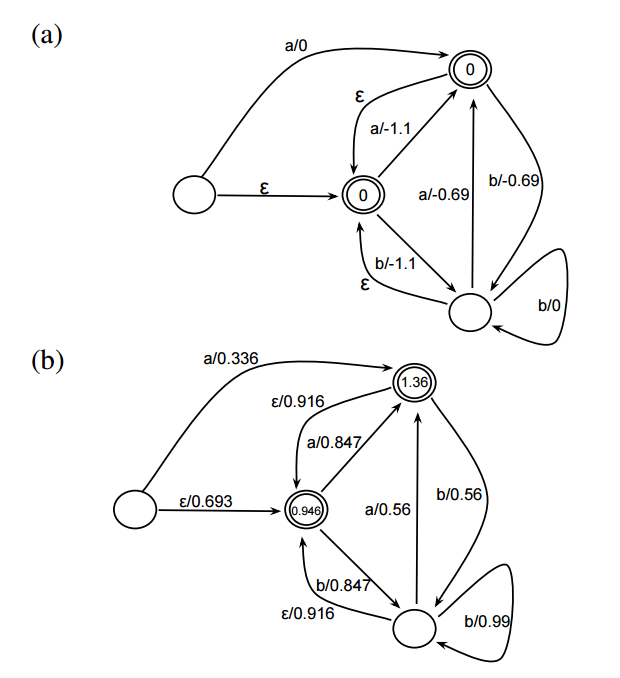
\includegraphics[width=7cm]{fsa}
  \end{center}
\end{frame}


\begin{frame}{Conclusion}
  
\end{frame}


\end{document}